\documentclass[tikz,border=2mm]{standalone}
\usepackage{ifthen}
\usepackage{amsmath} % 引入amsmath包以支持更复杂的数学表达式
\tikzset{global scale/.style={
    	scale=#1,
    	every node/.append style={scale=#1}
  	}
}

\[
f(x) = \frac{x^2 + 1}{\sqrt{x}} + \sin(x)
\]

\begin{document}
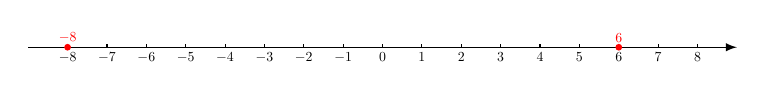
\begin{tikzpicture}[global scale = 0.5]


  	\draw [black, -latex] (-9,0) -- (9,0); 
	\foreach \x in {-8, ..., 8}
		\draw (\x cm,2pt) -- (\x cm,0pt) node[anchor=north] {$\x$};
	\foreach \n in {-8, 6}
		\draw [red, fill=red] (\n, 0) circle(2pt) node [above] {$\n$}; 
\end{tikzpicture}    
\end{document}
